\documentclass[nostatus,
%aspectratio=1610
]{MFHpresentation}
\usepackage{MFHcolours}
\usepackage{MFHscience}
\usepackage{MFHabbr}
\usetikzlibrary{positioning,arrows,backgrounds,fit,calc,tikzmark}
\usepackage{fontawesome}
\usepackage{multirow}
\usepackage{bbold}
\usepackage{bm}
\usepackage{marvosym}
\usepackage{ifthen}
\usepackage{transparent}

\usetheme{MFHepfl}

%------------------------------------------------------------------

\newcommand{\matmat}{\raisebox{-0.35em}{
\includegraphics[height=1.45em]{img/matmat.png}}\xspace}

%------------------------------------------------------------------

\title{
    Error control in scientific modelling\\[-0.2em]
    \textcolor{black}{\smaller[1.5] (with a focus on eigenvalue problems)}
}
\author{Michael F. Herbst, Niklas Schmitz}
\date[21.09.23]{21 September 2023}

\institute{Mathematics for Materials Modelling (\href{https://matmat.org}{\texttt{matmat.org}}), EPFL}

\titlegraphic{
    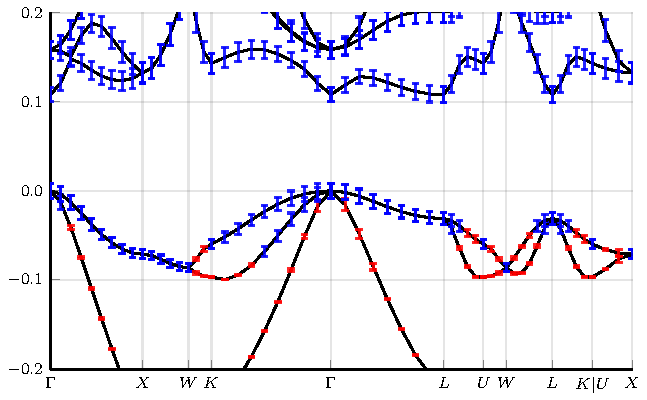
\includegraphics[width=0.4\textwidth]{img/si_band_errors.pdf}
    \qquad
    
\includegraphics[width=0.25\textwidth]{img/matmat.png}
}

\begin{document}
\setbeamerfont{footnote}{size=\tiny}

\showlogotrue
\begin{frame}[plain]
 \titlepage
 \addtocounter{framenumber}{-1}
\end{frame}

\showlogofalse
\begin{frame}{Leading thought}
    \begin{center}
        \alert{
            All computation is wrong, only some is useful.
        }
    \end{center}
    \vspace{4em}
    \begin{center}
        So far so obvious, but to what extend should one care?\\[1em]
    \visible<2>{
        \textcolor{grey5}{\smaller Or: Why should I devote a full semester to this topic?}
    }
    \end{center}
\end{frame}

\begin{frame}{Why care ? \quad Let's say your future job involves to \ldots}
    \begin{columns}[T]
        \smaller
    \begin{column}{0.3\textwidth}
    \begin{block}{Launch a rocket}
        \begin{center}
        \begin{tikzpicture}
            \node at (0, 0) {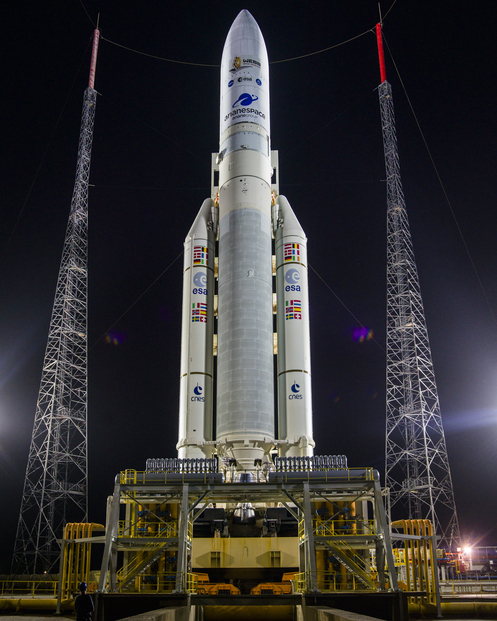
\includegraphics[width=0.8\textwidth]{img/disasters/Ariane_5.jpg}};
            \only<2->{\node [fill=white,rotate=40]  at (0, 0) {\alert{Self-destructed}};}
        \end{tikzpicture}
        \end{center}
        \visible<2->{
        \begin{itemize}
            \item June 1996
            \item Ariane 5 test
            \item 500 million dollar
            \visible<3->{
                \item \alert{floating point conversion error}
            }
        \end{itemize}
        }
    \end{block}
    \end{column}

    \begin{column}{0.3\textwidth}
    \begin{block}{Build an oil rig}
        \begin{center}
            \begin{tikzpicture}
                \node at (0, 0) {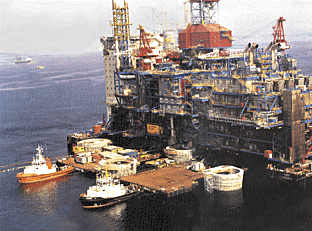
\includegraphics[width=\textwidth]{img/disasters/sleipner.png}};
                \only<2->{\node [fill=white,rotate=40]  at (0, 0) {\alert{Broken and sunken}};}
        \end{tikzpicture}
        \end{center}
        \visible<2->{
        \begin{itemize}
            \item August 1991
            \item Sleipner A offshore platform
            \item 1 billion dollar
            \visible<3->{
            \item \alert{Too crude discretisation}
            }
        \end{itemize}
        }
    \vspace{0.7em}
    \end{block}
    \end{column}

    \begin{column}{0.3\textwidth}
    \begin{block}{Intercept a missile}
        \begin{tikzpicture}
            \node at (0, 0) {
                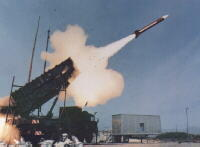
\includegraphics[width=\textwidth]{img/disasters/patriot.jpg}
            };
            \only<2->{\node [fill=white,rotate=40]  at (0, 0) {\alert{Missed Iranian missile}};}
        \end{tikzpicture}
        \visible<2->{
            \vspace{-1.0em}
        \begin{itemize}
            \item February 1991
            \item Patriot missile failure
            \item 28 soldiers killed, 100 injured
            \visible<3->{
            \item \alert{floating point conversion error}
            }
        \end{itemize}
        }
    \end{block}
    \end{column}
    \end{columns}

    \visible<3>{
    \vspace{1.0em}
    \begin{itemize}
            \smaller[2]
        \item See website of Douglas N. Arnold for more details:
            \url{https://www-users.cse.umn.edu/~arnold/disasters/disasters.html}
    \end{itemize}
    }
\end{frame}

\begin{frame}{Ok, so these are the extreme cases, right?}
    \begin{center}
        \larger
        \alert{Brainstorming:} Sources of error in scientific simulations
    \end{center}
    \vspace{3.0em}
    \visible<2>{
    \begin{itemize}
        \item Model
        \item Numerics \textcolor{grey5}{\smaller (discretisation / basis set, algorithm, arithmetic)}
        \item Implementation
        \item Hardware \textcolor{grey5}{\smaller (CPUs have bugs!)}
    \end{itemize}
    }
\end{frame}

\begin{frame}{Motivation in the \matmat group}
    \begin{itemize}
        \item \alert{21st century challenges}:
            \begin{itemize}
                \vspace{-0.3em}
                \item Renewable energy, green chemistry, health care \ldots
            \end{itemize}
        \vspace{0.2em}
        \item Current solutions limited by properties of available materials
            \begin{itemize}
                \vspace{-0.3em}
                \item[$\Rightarrow$] Innovation driven by \alert{discovering new materials}
            \end{itemize}
        \vspace{0.2em}
        \item Crucial tool: \alert{Computational materials discovery}
            \begin{itemize}
                \vspace{-0.3em}
                \item Systematic simulations on \alert{$\simeq 10^4 - 10^6$ compounds}
                \vspace{-0.3em}
                \item Complemented by data-driven approaches
                \vspace{-0.3em}
                \item \alert{Noteworthy share} of world's supercomputing resources
            \end{itemize}
    \end{itemize}
    \vspace{0.2em}
    \definecolor{pgray}{rgb}{0.169,0.169,0.251}
    \begin{center}
        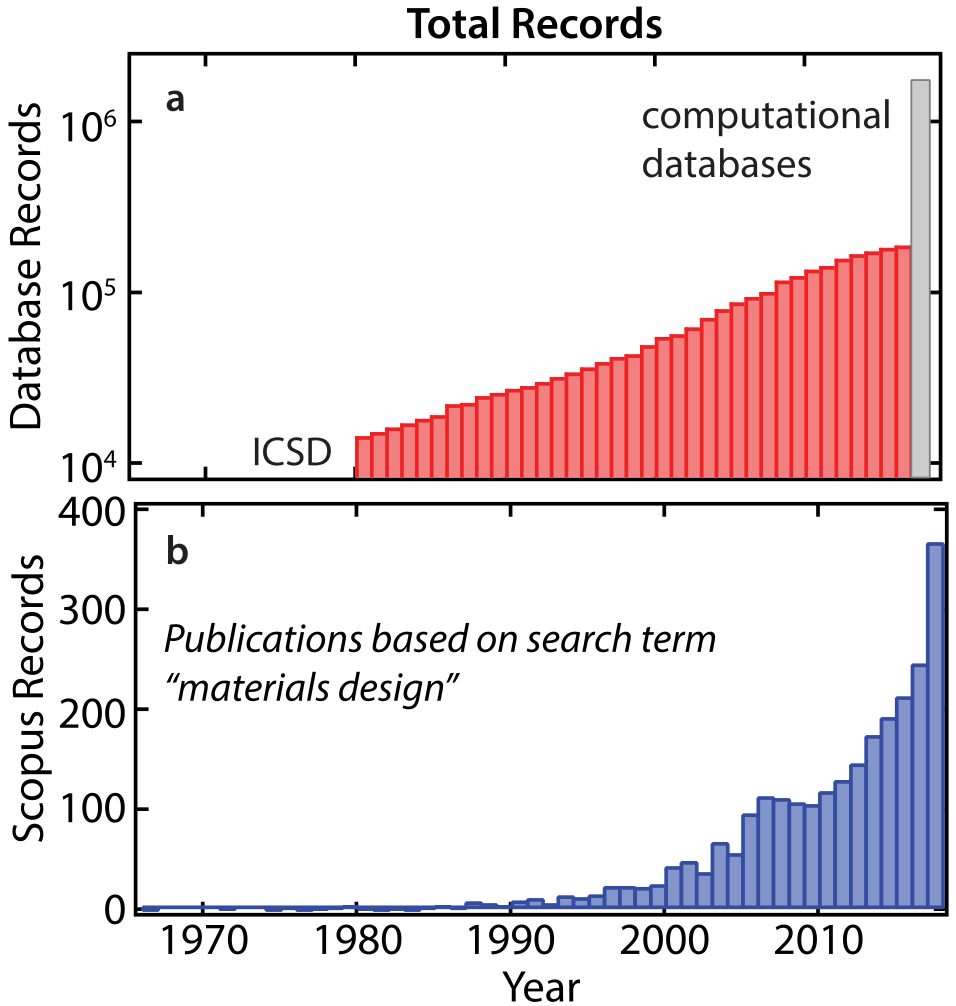
\includegraphics[height=3.3cm]{img/intro/roadmap-growth.png}
        \hspace{1.5em}
        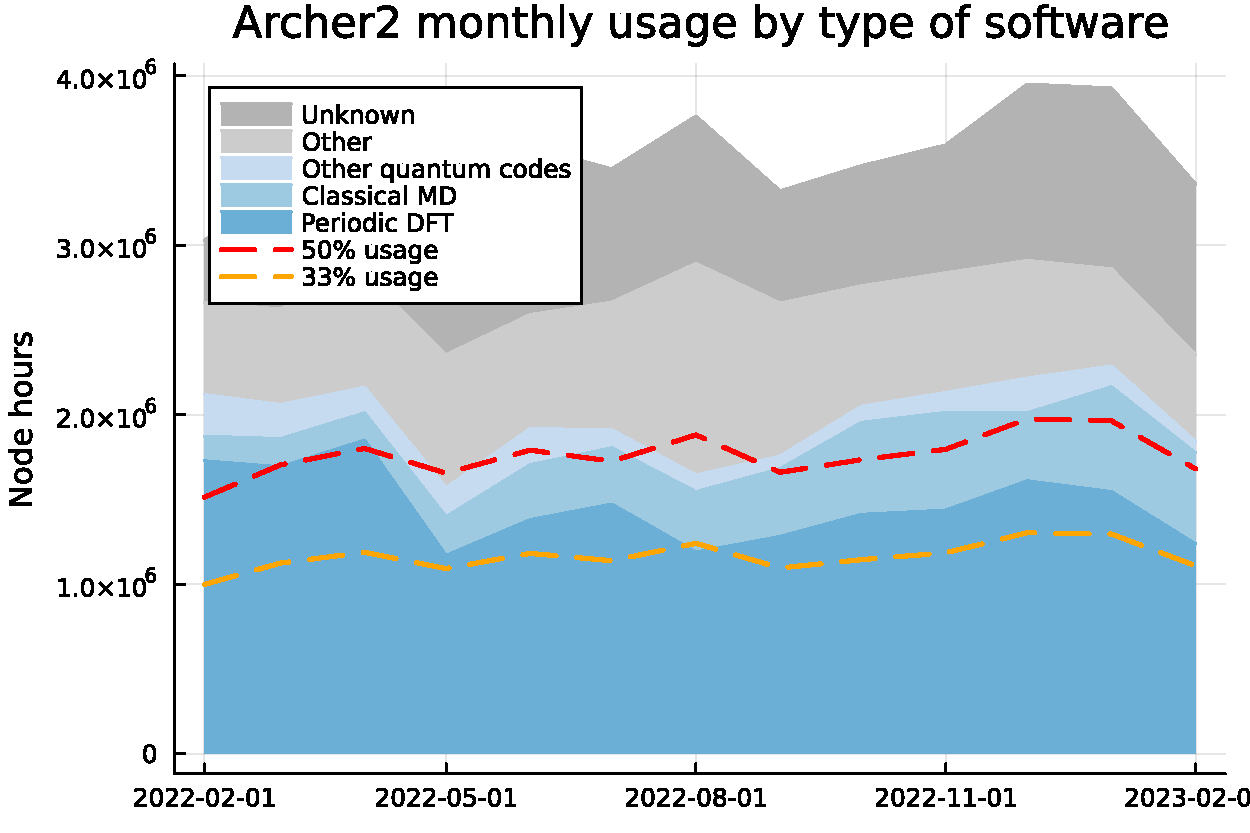
\includegraphics[height=3.3cm]{img/intro/archer_usage.pdf}
    \end{center}
   \vspace{-1.3em}
   \rule{4.5cm}{0.5pt}\\[-0.5em]
   {\tiny \href{http://dx.doi.org/10.1088/1361-6463/aad926}{%
       K. Alberi \textit{et. al.} J. Phys. D, \textbf{52}, 013001 (2019).}}
\end{frame}

\begin{frame}{Sketch of high-throughput workflows}
    \widenframe[4em]{
        \vspace{-0.2em}
        \begin{columns}
        \begin{column}{0.45\textwidth}
        \begin{lpic}[r(2.5cm)]{./img/intro/funnel.png(.125)}
        \lbl[l]{232,153;$\Big\}$\smaller[2.5] DFT PBE stability}
        \lbl[l]{203, 95;\smaller[2.5]DFT PBE band gap}
        \lbl[l]{187, 60;\smaller[2.5]Hybrid-DFT band gap}
        \lbl[l]{175, 25;\smaller[2.5]Beyond DFT}
        \end{lpic}\\[-0.7em]
        {\smaller[2.5] Design funnel for photovoltaic materials}
        \end{column}
        \begin{column}{0.55\textwidth}
        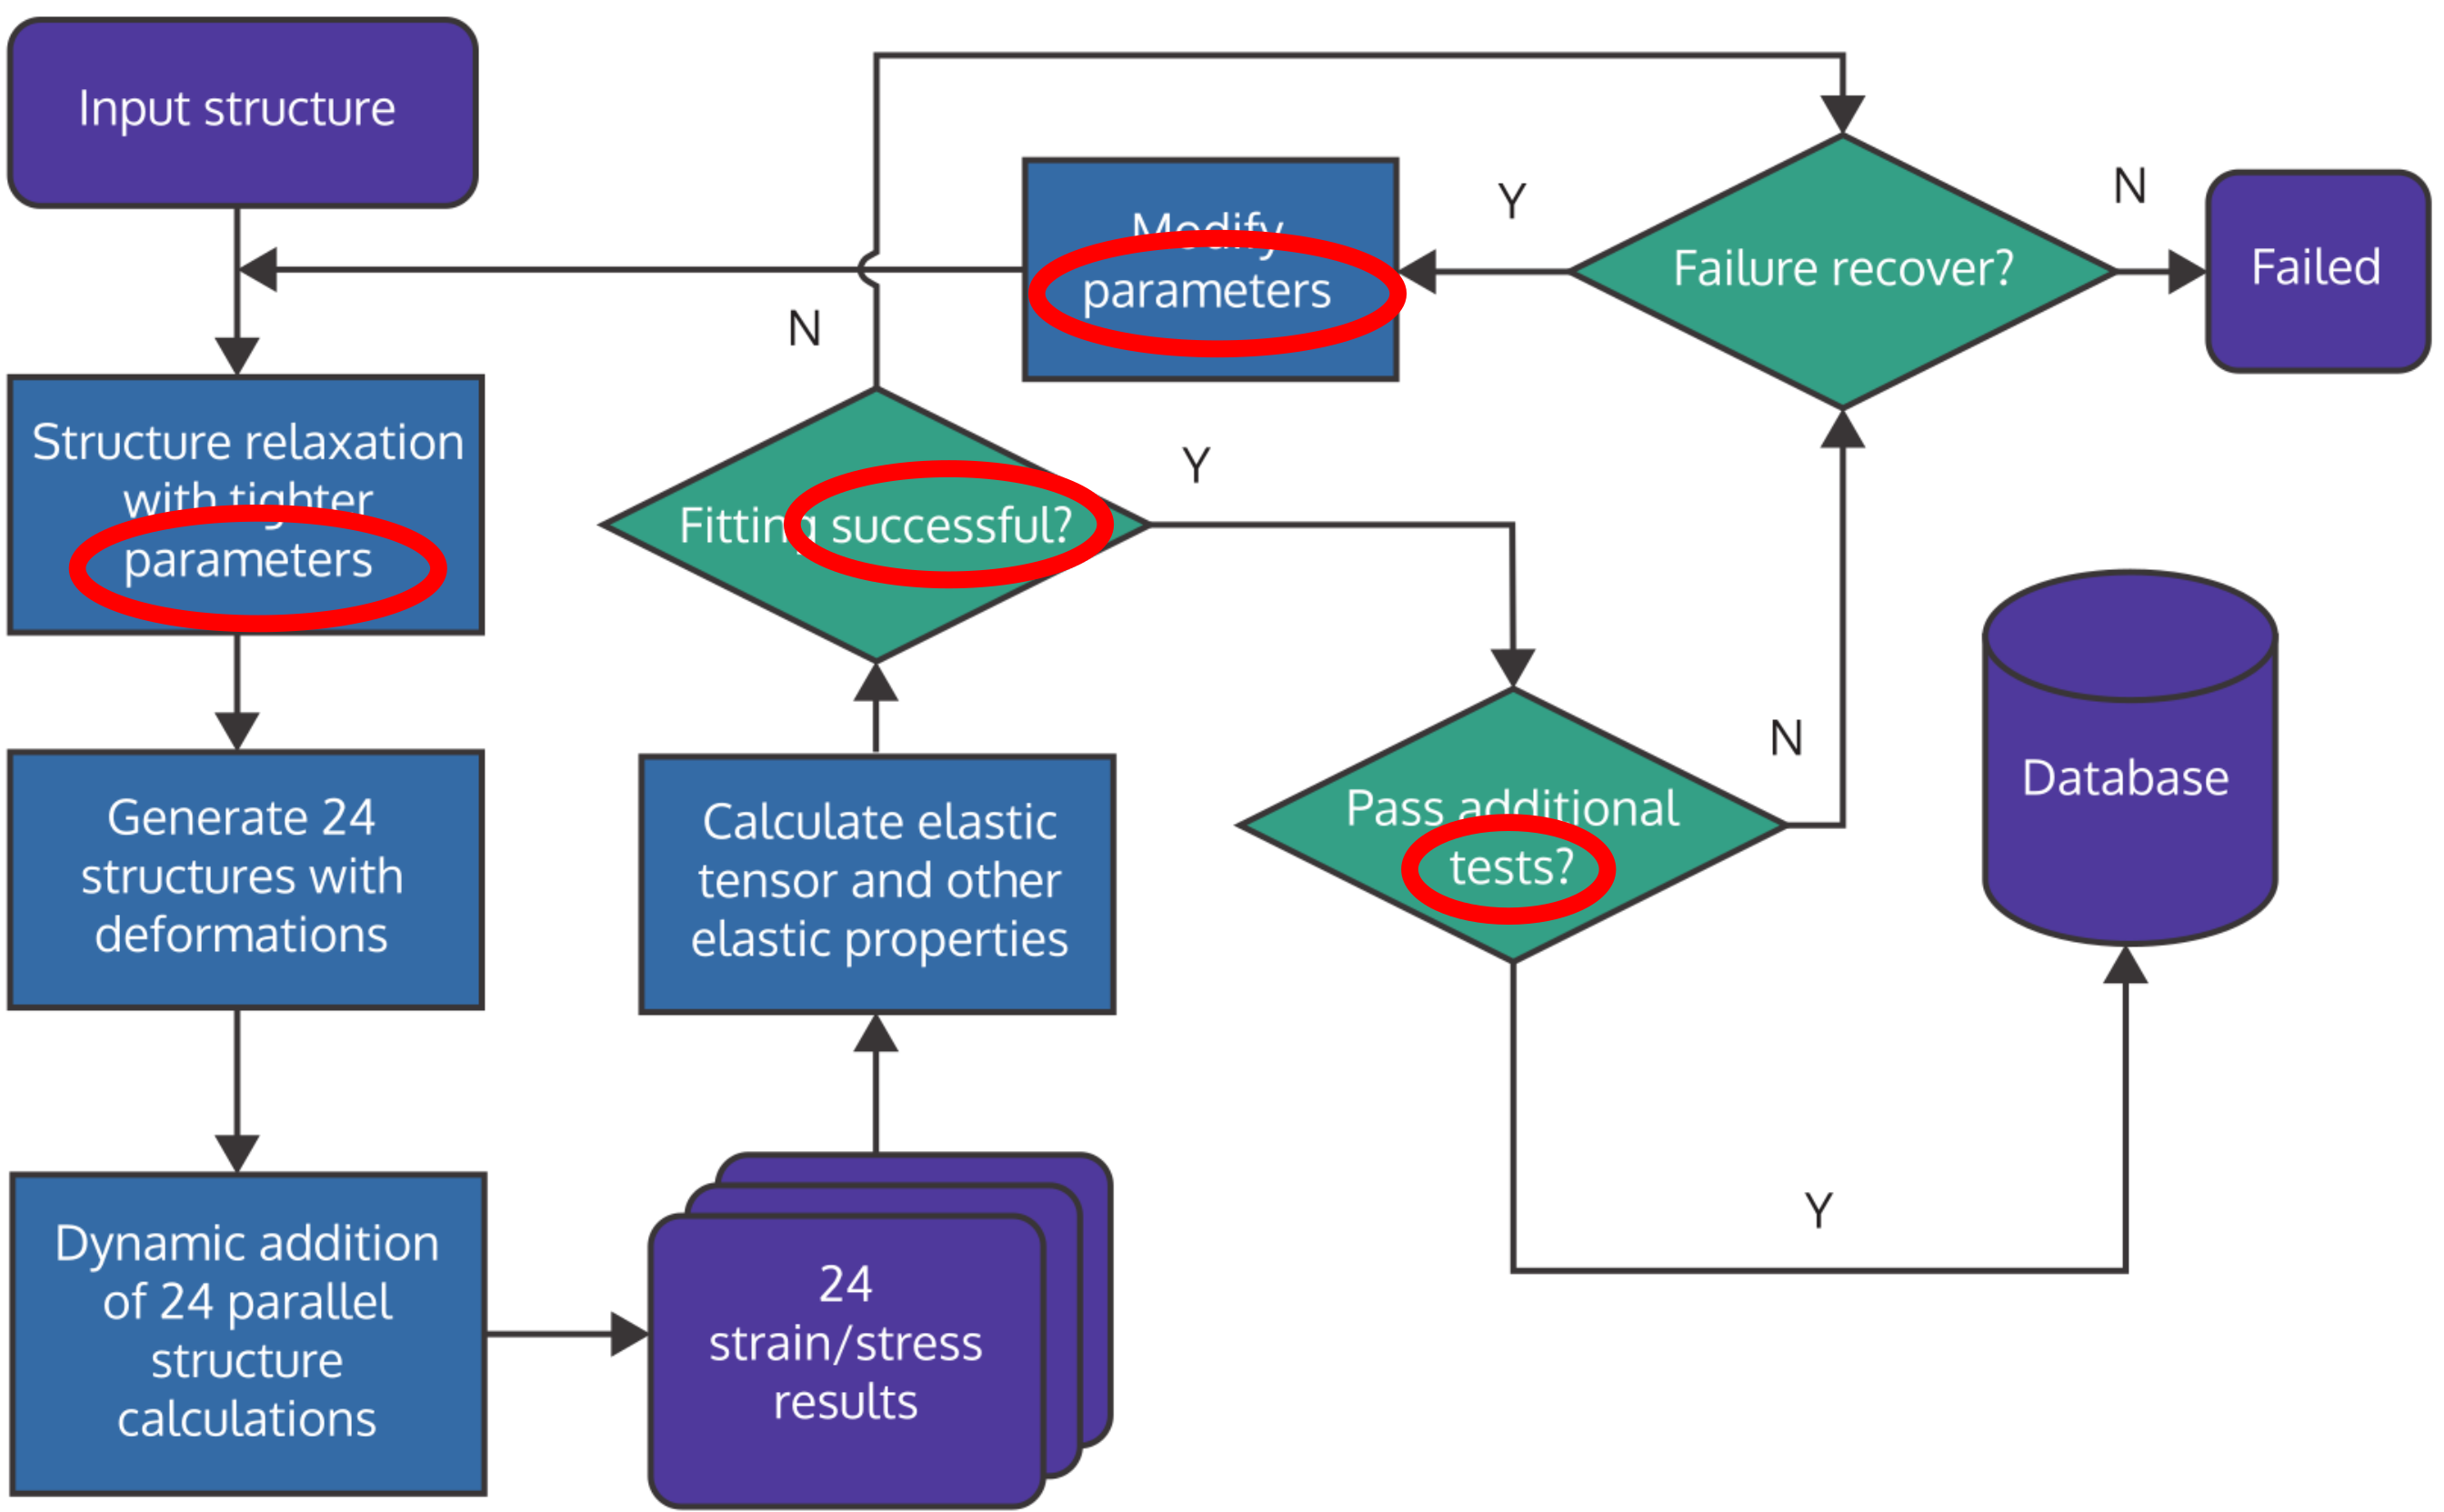
\includegraphics[width=5.0cm]{./img/intro/workflow_edit_parameters.png}%
        \\[-0.5em]
        {\smaller[2.5] Workflow for computing elasticity tensors}
        \end{column}
        \end{columns}
    }
    \vspace{-0.1em}
    \begin{itemize}
        \item Many parameters to choose \textcolor{grey5}{(algorithms, tolerances, models)}
            \begin{itemize}
                \vspace{-0.4em}
                \item Elaborate heuristics: \alert{Failure rate $\simeq 1\%$}
                \vspace{-0.4em}
                \item Still: \alert{Thousands} of failed calculations
                \vspace{-0.4em}
                \item[$\Rightarrow$] \alert{Wasted resources} \& increased human attention
                    \textcolor{grey5}{\smaller (limits througput)}
            \end{itemize}
        % \vspace{0.1em}
        % \item Carbon footprint? More complex design spaces?
        \vspace{0.2em}
        \item \textbf{Goal} in \matmat group: \alert{Self-adapting black-box algorithms}
            \begin{itemize}
                \vspace{-0.4em}
                \item Transform \alert{empirical wisdom} to built-in \alert{convergence guarantees}
                \vspace{-0.4em}
                \item Requires: Uncertainty quantification \& error estimation
                \vspace{-0.4em}
                \item[$\Rightarrow$] Understand \alert{where and how} to spend efforts best
            \end{itemize}
   \end{itemize}
   \vspace{-0.8em}
   \rule{4.5cm}{0.5pt}\\[-0.5em]
   {\tiny G.~Hautier Comput. Mater. Sci. \textbf{164}, 108 (2019);
       L.~Himanen \textit{et. al.} Adv. Science \textbf{6}, 1900808 (2019).}
\end{frame}

\begin{frame}{Broader vision: Robust \& error-controlled simulations}
\begin{itemize}
    \item Error control $=$ \alert{Track simulation uncertainties}:
        \begin{itemize}
            \vspace{-0.30em}
            \item Self-adapting simulations with mathematical guarantees
            \vspace{-0.30em}
            \item Integrate with error propagation efforts for surrogates%
                \footnote{F.~Musil, A.~Grisafi \emph{et. al.} J. Chem. Theo. Comput. \textbf{15}, 2 (2019).}
            \vspace{-0.30em}
            \item [$\Rightarrow$] Byproducts: Data quality control,
                accelerated design%
                % \footnote{G.~Houchins and V.~Viswanathan MRS Bulletin \textbf{44}, 204 (2019).}
        \end{itemize}

    \vspace{0.3em}
    \item Error control $=$ \alert{Learn missing physics}:
        \begin{itemize}
            \vspace{-0.30em}
            \item Data-enhanced models, active learning
            \vspace{-0.30em}
            \item Integration with experiment {\color{grey5} (autonomous discovery)}
            \vspace{-0.30em}
            \item [$\Rightarrow$] Exploit high-fidelity experimental, beyond-DFT data
        \end{itemize}

    \vspace{0.3em}
    \item Error control $=$ \alert{Leverage inexactness}:
        \begin{itemize}
            \vspace{-0.30em}
            \item Error balancing: Optimal adaptive parameter selection
            \vspace{-0.30em}
            \item Randomised methods, selective precision {\color{grey5} (16-bit, FPGA)}
                % Error control and multi-fidelity approaches pretty much unexplored
                % in practical setting
            \vspace{-0.30em}
            \item Multi-fidelity approaches {\color{grey5} (reduced basis, surrogates)}
        \end{itemize}

    \vspace{0.3em}
    \item[$\Rightarrow$] Understand \alert{where and how} to spend efforts best
    \vspace{-0.3em}
    \item[$\Rightarrow$] Realm of mathematical research
\end{itemize}
\vspace{1em}
\end{frame}


\begin{frame}{Questions ?}
    \begin{center}
        \huge{Questions ?}
    \end{center}
\end{frame}

\begin{frame}{Focus of the course: Eigenvalue problems}
    \begin{itemize}
        \item Eigenvalue problems are ubiquitous, e.g.
        \vspace{2em}
        \item \alert{Vibrations of structures}
            \begin{itemize}
                \item Tacoma narrows bridge collapse 1940
                \item London millennium bridge construction flaw
            \end{itemize}
        \vspace{1em}
        \item \alert{Quantum states} \textcolor{grey5}{\smaller (details follow)}
        \vspace{1em}
        \item Tight relation to \alert{linear problems \& PDEs}
            \begin{itemize}
                \item Convergence analysis (CG, iterative methods)
                \item Quantum mechanics
                \item Close relation to solving PDEs
                    \textcolor{grey5}{\smaller (details follow)}
            \end{itemize}
    \end{itemize}
\end{frame}

\begin{frame}{Structure of the course}
    \begin{itemize}
        \item \alert{Moodle:} \url{https://go.epfl.ch/error-control}
        \vspace{-0.3em}
    \item \alert{ED Forum:} Announcements \& \alert{student-driven} discussion
        \vspace{1.0em}
        \item Lectures split into two rough segments
            \begin{itemize}
                \vspace{-0.3em}
                \item \alert{First half:} Matrix eigenvalue problems \& floating-point error
                \vspace{-0.3em}
                \item \alert{Second half:} Operator theory \& discretisation error
                \vspace{-0.3em}
                \item \alert{Addendum:} Statistical method for error control
                    \textcolor{grey5}{(if time)}
                \vspace{-0.3em}
                \item \alert{Notes:} \url{https://teaching.matmat.org/error-control}
            \end{itemize}
        \vspace{1.0em}
        \item Attendance of exercises is \alert{expected} \textcolor{grey5}{(introduces new material!)}
            \begin{itemize}
                \vspace{-0.3em}
                \item Discussion follows weekly exercise sheet
            \end{itemize}
    \end{itemize}
\end{frame}

\begin{frame}{Course evaluation}
    \setlength{\leftmargini}{0ex}
    \setlength{\leftmarginii}{4ex}
    \begin{itemize}
        \item Marked semester project \textcolor{grey5}{($1/3$ of grade)}
        \item Project interview \& oral exam \textcolor{grey5}{($2/3$ of grade)}
        \item Project done in \alert{teams of $2-3$ students}.
        \item Interdisciplinary teams are highly recommended
        \vspace{1.5em}
        \item Working on the projects
            \alert{requires substantial time outside class}
            \begin{itemize}
            \vspace{-0.3em}
            \item[$\Rightarrow$] We will setup \alert{survey} in \textbf{week 2} to \alert{aid formation of groups}
            \end{itemize}
    \end{itemize}
\end{frame}

\begin{frame}{Details on the exercises \& problem sheets}
    \begin{itemize}
        \item One problem sheet per week from moodle: \url{https://go.epfl.ch/error-control}
        \vspace{1em}
        \item Exercise sheets: Not handed in or marked
            \begin{itemize}
                \vspace{-0.3em}
                \item Project groups \alert{take turns to present sheet}
                \vspace{-0.3em}
                \item \alert{Not marked}; group just presents status of their work
                \vspace{-0.3em}
                \item Class/tutors give feedback on presented results
            \end{itemize}
        \vspace{1em}
        \item Initial exercises classes will be denser
        \vspace{-0.3em}
        \item Later exercise classes provide time to work on the project
        \vspace{1em}
    \item \alert{Important:}
        \begin{itemize}
            \vspace{-0.3em}
            \item \textbf{Bring your laptop} to the exercise sessions
            \vspace{-0.3em}
            \item \textbf{Install \julia} programming language \textbf{beforehand}
            \vspace{-0.3em}
            \item[$\Rightarrow$] See \alert{instructions on moodle}
        \end{itemize}
    \end{itemize}
\end{frame}

\begin{frame}{Details on the project}
    \begin{itemize}
        \vspace{-0.3em}
        \item Project is essentially a larger problem sheet
        \vspace{-0.3em}
        \item One joint solution is submitted by each group
        \vspace{-0.3em}
        \item Responsibilities should be shared equally.
        \vspace{1.0em}
        \item During the oral exam \textcolor{grey5}{(about half the time)}
            \begin{itemize}
                \vspace{-0.3em}
                \item Presentation of the problem sheet by student
                \vspace{-0.3em}
                \item Targeted follow-up questions
                \vspace{-0.3em}
                \item \textcolor{grey5}{(The other half of the oral
                    is about general course understanding)}
            \end{itemize}
        \vspace{1.0em}
        \item Project evaluation criteria:
            \begin{itemize}
                \vspace{-0.3em}
                \item See document on moodle
            \end{itemize}
        \vspace{1.0em}
        \item Each group member obtains an \alert{individual mark}.
    \end{itemize}
\end{frame}

\begin{frame}{Topic of the semester project}
    \begin{itemize}
        \item Topic: \alert{Band structures with guaranteed error bars}
            \begin{itemize}
                \vspace{-0.5em}
                \item Handout: 24st October \textcolor{grey5}{(tentative)}
                \vspace{-0.5em}
                \item Duration: 2 months, i.e.~projected deadline: \textbf{19 December}
            \end{itemize}
        \vspace{1.5em}
        \begin{center}
        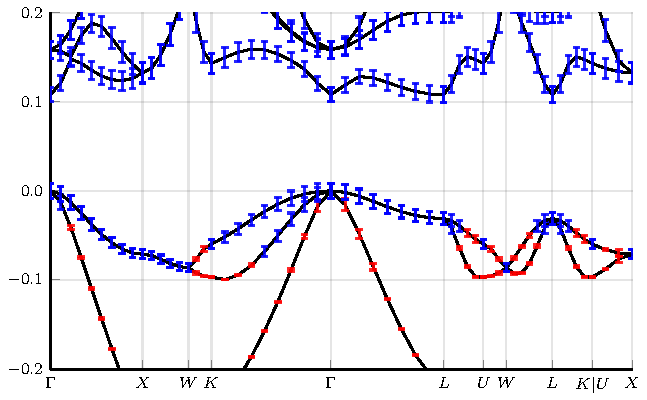
\includegraphics[width=0.7\textwidth]{img/si_band_errors.pdf}
        \end{center}
        \vspace{0.5em}
        \item Let's have a brief look at last year's projects \ldots
    \end{itemize}
\end{frame}

\begin{frame}{Group dynamics and mediation}
    \begin{itemize}
        \item Team work involves people
        \item People means tensions
            \begin{itemize}
                \vspace{-0.3em}
                \item \ldots and potentially unfair distribution of work
                \vspace{-0.3em}
                \item This is not unusual in academic and industry teams !
            \end{itemize}
        \vspace{1.0em}
        \item Additional \alert{learning goals of this course}:
            \begin{itemize}
                \item Learning to distribute work
                \item Learning to coordinate as a team
                \item Learning to resolve conflicts
            \end{itemize}
        \vspace{1.0em}
            \item \alert{You are not on your own}
                \begin{itemize}
                \vspace{-0.3em}
                \item We can provide support and mediate
                \vspace{-0.3em}
                \item Survey around \textbf{week 4}: \alert{All good ? (y/n)}
                \end{itemize}
            \vspace{0.5em}
            \item \textbf{But} we cannot assist you if you don't reach out
                \linebreak
                \textbf{Hint:}  After the exam is too late
    \end{itemize}
\end{frame}

\begin{frame}{Questions ?}
    \begin{center}
        \huge{Questions ?}
    \end{center}
\end{frame}

\begin{frame}{Your background \& prior knowledge}
    \begin{center}
        \LARGE{Your background and prior knowledge}
    \end{center}
\end{frame}

\begin{frame}{Vector spaces}
    \noindent
    Which of the following things is a \alert{vector space} over $\R$
    \vspace{1em}
    \begin{enumerate}
        \item $\R^n = \{(x_1, \ldots, x_n)^T , x_i \in \R \}$
        \item $\mathcal{F}(D, \R) = \{f : D \to \R\}$,
            the set of all functions from $D$ to $\R$.
        \item $\R^{n\times n}$: The set of all matrices
    \end{enumerate}
    \vspace{1em}
    \visible<2>{\alert{Answer:} All of them!}
\end{frame}

\begin{frame}{Inner products}
    \noindent
    Given vectors $x,y,z$ from an $\C$-vector space $V$.
    What makes an \alert{inner product}?
    \visible<2>{
        \vspace{1em}
        \begin{itemize}
            \item $\langle x, x \rangle \geq 0$
            \item $\langle x, y \rangle = \overline{\langle y, x \rangle}$
            \item $\langle x, \alpha y + \beta z \rangle
                = \alpha \langle x, y \rangle
                + \beta \langle x, z \rangle$
        \end{itemize}
        \vspace{1em}
        Examples:
        \begin{itemize}
            \item 
        $\langle x, y \rangle = x^H y = \overline{x^T} y = \sum_{x=1}^n \overline{x_i} y_i$ for vectors $x,y \in \C^n$
        \item
        $\langle A, B \rangle_F = A^H B = \tr(A^H B)$ 
        for matrices $A,B \in \C^{n\times n}$
        \end{itemize}
    }
\end{frame}

\begin{frame}{Norms}
    \noindent
    Which of these statements is true:
    \vspace{1em}
    \begin{enumerate}
        \item If $\langle x, y\rangle$ is an inner product,
            then $\norm{x} = \sqrt{\langle x, x \rangle}$ is a norm
        \item If $\langle x, y\rangle$ is an inner product
            and $\norm{x} = \sqrt{\langle x, x \rangle}$, then
            \[ \langle x, y \rangle < \norm{x} \norm{y} \]
        \item If $\norm{x}$ is a norm, there exists an inner product
            $\langle x, y\rangle$, such that $\norm{x} = \sqrt{\langle x, x \rangle}$
        \item Every norm satisfies the triangle inequality
            \[ \norm{x + y} \leq \norm{x} + \norm{y} \]
    \end{enumerate}
    \vspace{1em}
    \visible<2>{\alert{Answer:} 1 and 4 are true, 2 and 3 are false.
        2 is almost true the correct version is
        \[ \langle x, y \rangle \leq \norm{x} \norm{y} \qquad \text{Cauchy-Schwarz}\]
    }
\end{frame}

\begin{frame}{Diagonalisation algorithms}
    \noindent Which iterative diagonalisation algorithms do you know?\\
    \vspace{1em}
    \noindent Who has studied before:
    \vspace{1em}
    \begin{itemize}
        \visible<2->{\item Power method}
        \visible<3->{\item Inverse power method}
        \visible<4->{\item Rayleigh-quotient iteration}
        \visible<5->{\item LOPCG}
    \end{itemize}
\end{frame}



% Sobolev spaces
% Hilbert spaces
% Numerical analysis
% PDE discretisations
% a posteriori error
% spectral theorem
% operators
% spectral theory
% diagonalisation algorithms
% Quantum mechanics
% Harmonic oscillator
% Plane waves
% Programming
% Julia

\begin{frame}{I need a volunteer}
    \begin{itemize}
        \item \textbf{Your job:} Take pictures of blackboards
    \end{itemize}
\end{frame}

\end{document}
